\scanpage{22}
$\mathcal E^{2n}$ \deleted{est engendré par} \inserted{admet la \uline{base}} $L_0^n$,
\inserted{(pour un $L_0$ de Lefschetz fixé)}
\deleted{$\mathcal E^{-2n}$ \unsure{engendré} par $\unsure{\Lambda_0^n|\Lambda^n}$,}
\deleted{pour un choix de $(L,\Lambda)$.}
\deleted{de $\mathcal E^{2n}$, \illegible{2} de $L'$.}
Or.\,--- où, si $L'$ est un autre élément Lefschetzien
\figure{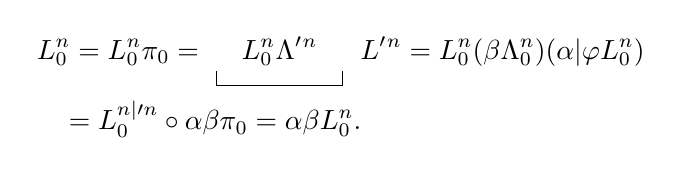
\begin{tikzpicture}
\node[anchor=base east] at(-.9,0){$\displaystyle L_0^n=L_0^n\pi_0=$};
\node[anchor=base] at(0,0){$\displaystyle L_0^n\Lambda'{}^n$};
\node[anchor=base west] at(.9,0){$\displaystyle L'{}^n=L_0^n(\beta\Lambda_0^n)(\unsure{\alpha|\varphi}L_0^n)$};
\draw(-.8,-.15)--(-.8,-.33)--(.8,-.33)--(.8,-.15);
\node[anchor=base west] at(-2.8,-.9){$\displaystyle =L_0^{\unsure{n|\prime n}}\circ\alpha\beta\pi_0=\alpha\beta L_0^n.$};
\end{tikzpicture}}
ce qui prouve que $\alpha\beta=1$, donc $\alpha$ et $\beta$ inversibles, donc \deleted{\unsure{pour}} $L_0^{\unsure{\prime n|n}}$ et $\Lambda_0^{\unsure{\prime n|n}}$ sont des bases de $\mathcal E^{(2n)}$ et $\mathcal E^{(-2n)}$ respectivement.

D'où
\diagram{\begin{tikzcd}[ampersand replacement=\&,column sep=large]
L^{\unsure{\prime|*}}\ \text{Lefschetzien}\arrow[r,Rightarrow]\&L^n\ \text{\uline{une base de}}\ \mathcal E^{2n}
\end{tikzcd}}
\figure{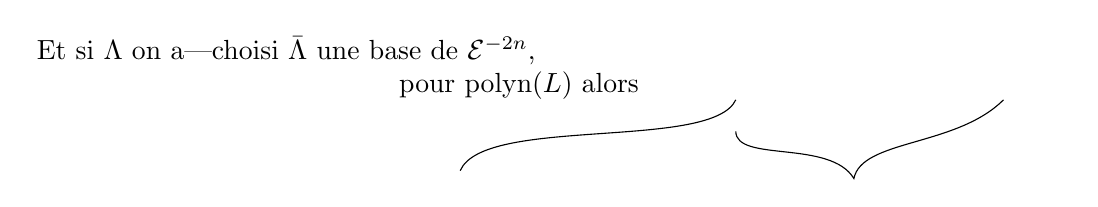
\begin{tikzpicture}[x=1cm,y=1cm]
\node[anchor=west,align=left,text width=13cm] at (0,1.1) {\inserted{Et si $\deleted{\unsure{\Lambda}}$ \unsure{on a|choisi} $\bar\Lambda$ une base de $\mathcal E^{-2n}$,\\\hspace*{4.6cm}\unsure{pour} \uline{\unsure{polyn}}$(L)$ \unsure{alors}}};
\draw (5.5,-.2) .. controls (5.8,.5) and (8.7,.05) .. (9,.7);
\draw (9,.3) .. controls (9,-.1) and (10.2,.2) .. (10.5,-.3) .. controls (10.6,.2) and (11.8,.1) .. (12.4,.7);
\end{tikzpicture}}
\margin{?}
On \unsure{veut|peut} prouver une réciproque, dans le cas où \deleted{$\unsure{\mathcal E}$} $\mathcal E$ est projectif de type fini sur $A$. \unsure{Ça|Ce} ne marche certainement pas tel quel, p.ex. pour $\mathcal E=\mathcal L(M^*)$, $M^*$ gradué à degrés $0\leq i\leq4$ ---.

Mais ça ne marche pas non plus pour les endom. associés aux élémts de degré $2$ d'une alg. de Lefschetz, pour la dim $6$

$\mathcal E$ engendré par $L,L'$ \inserted{\figure{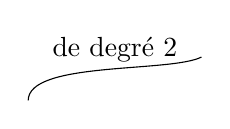
\begin{tikzpicture}
\node at(0,0){de degré $2$};
\draw(-1.1,-.65) .. controls(-1.1,-.15) and(.7,-.3) .. (1.1,-.1);
\end{tikzpicture}}} avec les relations
\[
L^4=0,\quad L'^2-LL'=0,\quad L^2L'-L^3=0,\quad L^3L'=0,\qquad\text{de base}
\]
\diagram{\begin{array}{r c||c||c||c}
&1&L,L'&L^2,LL'&L^3\\\cline{2-5}
\text{degré}&0&2&4&
\end{array}}
\margin{\figure{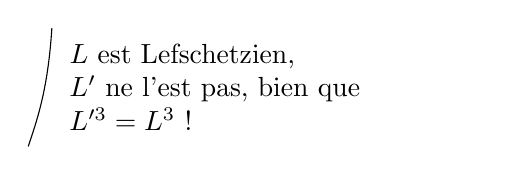
\begin{tikzpicture}
\draw(.3,1.5) .. controls(.25,.7) and(.1,.3) .. (0,0);
\node[anchor=west,align=left,text width=5.1cm] at(.4,.75){$L$ est Lefschetzien,\\$L'$ ne l'est pas, bien que\\$L'^3=L^3$ !};
\end{tikzpicture}}}
\mspage{21}
